\documentclass[11pt]{article}
\usepackage{blindtext}
\usepackage{tikz}
\usepackage{varwidth}
\usepackage{capt-of}  
\usepackage{wrapfig}
\usepackage{caption}
\usepackage{subcaption}
\usepackage{amsmath}
\usepackage{amssymb}
\usepackage{bbm}
\usepackage{wrapfig}
\usepackage{parskip}
\usepackage{hyperref}%hyperrects
\usepackage[a4paper, margin=2cm,headsep=6pt]{geometry}
\usepackage{lineno}
\usepackage[english]{babel}
\usepackage{graphicx}
\usepackage{float}
\usepackage{csquotes}
\usepackage{fancyhdr}
\setlength{\headheight}{14pt}
\usepackage{placeins}
\usepackage{booktabs,tabularx}
\usepackage[font=small,labelfont=bf]{caption}
\usepackage{graphicx}
\usepackage[backend=bibtex,style=authoryear]{biblatex}
\bibliography{minireport.bib}
\hypersetup{
colorlinks=true,
linkcolor=blue,
urlcolor=blue,
citecolor=blue,
}

\setlength{\parskip}{\medskipamount}
\makeatletter 
\newcommand{\@minipagerestore}{
\setlength{\parindent}{15pt}
%\setlength{\parskip}{\medskipamount}
}
\newcommand{\soptitle}{Comparing Mathematical Models for Bacterial Growth Curves Fitting}
\pagestyle{fancy}
\linespread{2}
\fancyhead[R]{CID YY5819}
\fancyhead[L]{Yuchen Yang}


\begin{document}
\begin{titlepage}
\begin{center}
\hrule
\vspace{2pt}
\hrule
\vspace{2cm}
\LARGE {\bf \underline{Mini Project}}\\
\vspace{2cm}
\huge{\bf \soptitle}\\
\large {\bf Word Count: 2953}\\
\vspace{8cm}
\LARGE {\bf Yuchen Yang}\\
\large {\bf MRes Computational Method for Ecology and Evolution}\\
\large {\bf Department of Life Sciences}\\
\large {\bf Imperial College London}\\
\large {\bf yuchen.yang19@imperial.ac.uk}
\vspace{2cm}
\end{center}
\hrule
\vspace{2pt}
\hrule
\end{titlepage}
\linenumbers
\section*{Abstract}
This study compares the Baranyi, Logistic, Gompertz, and the basic Polynomial(Cubic) model's behaviour in a bacterial growth data set using $AIC$, $\Delta AIC$, and $AIC weight$ (and reasons to exclude other indicators). The result indicates that the \textbf{Gompertz} model is the best model for fitting this general data set(regarded as best fit for a total of \textbf{182} times among other models, taking up \textbf{62.5\%} of the total data set groups), despite the fact that there are argument saying the more mechanistic Baranyi model would be better. The study also used a subset of \textbf{Tetraselmis tetrahele} in the data set to examine temperature's effect on model fitting's behaviour. The result from the Kruskal-Wallis Test indicates that models have shown a significant differences (Baranyi's $p-value = 0.001679$, Logistic's $p-value = 0.01684$, Gompertz's $p-value = 0.03801$, Polynomial's $p-value = 0.01672$) in their $AIC weight$ across different temperature groups. Finally, this study compared models' behaviour on the death phase of a growth curve and explore the reasons for those differences in performances.

\section{Introduction}
Mathematical models are used to understand and predict the growth of the bacterial population for quite a long time. Most bacterial growths in batch culture follow a distinct set of phases - lag phase, exponential phase and stationary phase, which would perfectly fit a sigmoid shape. The Gompertz model\parencite{gompertz1825xxiv} and the Logistic model \parencite{verhulst1838notice} are the most frequently used sigmoid models fitted to growth\parencite{tjorve2017use}. However, most of the time nowadays, taking measurement errors and the expected growth kinetics into consideration, food microbiology researches would use the logarithm of cell concentrations as raw data. Some of the papers are using those classical sigmoid growth models as above, but since the population is in the logarithm of the cell concentrations, the results are not as good\parencite{baranyi2011modelling}.
Baranyi also pointed out that the reason those two models, while being very popular and useful, has their limitations, especially in fitting bacterial data, is that the original model's curve does not remain sigmoid shape, but rather a monotone shape in log-space. Hence they could fail to capture the lag phases, and so that the use of such models are limited\parencite{baranyi2011modelling}.\\
It has been argued that the empirical models such as modified Gompertz and Logistic models were not as preferred as the more mechanistic models such as the Baranyi model even with the modifications for it to work better in log-space\parencite{juneja2009mathematical}. To compare and evaluate similarities and differences between the models behaviour on a general bacterial database, this study has chosen the Baranyi \parencite{baranyi1993non}, the Logistic, the Gompertz(both using the log-transformed formulation of Zwietering)\parencite{zwietering1990modeling} and the basic Polynomial(Cubic) model, from the most mechanistic to the least, to better understand the behavioural differences. \\
Aside from understand how different models perform in a fitting practice, it is also interesting to understand what are the co-variate's role in this. Will a model's performance differ across different co-variate groups? Understanding this would be helpful for researchers to find find appropriate models to use in future analysis based on the condition of the data set.
the Polynomial model is introduced mainly to benchmark models' behaviour on a fourth stage that has not been very often mentioned - death phase. Since A Cubic model have a declined phase at the end, it may be quite good at capturing decline in population size after some maximum value (the carrying capacity) has been reached (the "death phase" of population growth)\parencite{buchanan1918life}, it is also interesting to see how different models are behaving in that period.\\
To recap on the objectives:
\begin{itemize}
  \item This study would first compare the above-mentioned models' behaviour for a general bacterial data set, and determine which one fits better.
  \item This study would help to understand different co-variates' (specifically focus on temperature) effect on model fitting performance.
  \item This study will touch base on the death phase performances.
\end{itemize}


\section{Data}
\subsection{Basic Features}
The data set consists of data from multiple pieces of research, which contains measurements of change in biomass or number of cells of microbes over time and were collected through lab experiments across the world. the original data can be found in the \verb|Data| directory with the name \verb|LogisticGrowthData.csv|, detailed column metadata could be seen in \verb|LogisticGrowthMetaData.csv|. The two main fields of interest are called \verb|PopBio|(abundance), and \verb|Time|.\\
The data set consists of 4387 rows of data from 10 pieces of research, covering a total of 17 temperature groups from 0 to 37$^\circ C$, 45 species, and 18 mediums. At the first glance, the \emph{min} of the \verb|Time| is -25.2632, the \emph{min} of the \verb|PopBio| is -668.284, suggesting further data wrangling is required, but there are no missing values in the data.
\subsection{Pre-Processing}
\subsubsection{Re-Calibrate}
The data set is grouped into 305 groups based on its \verb|Temp|, \verb|Species|, \verb|Medium|, \verb|Citation|, and \verb|Rep| to better facilitate the study. The group sample size is rather small, with a \emph{mean} of 14.36066 and a \emph{median} of 12. Furthermore, each group's starting point \verb|O(T_{0}, N_{0})| is used as a reference to move the whole group's data to the origin to get rid of any negative values and make better sense.
\subsubsection{Logarithm}
Since all the model we have used is either designed for the log-space or being log-transformed. To better unify the results and deal with measurement errors, etc., a new column called \verb|logPopBio|, which is the natural log of the original \verb|PopBio|, is added and used for all future analysis.
\subsubsection{Death Phase}
To better understand the fitting performance of all models during the "death phase", which is a decline of the population after reaching the maximum population, a column named \verb|deathPhase| is added. By default the value is $0$, and when $\frac{N_{max} - N_{tlast}}{N_{max}-N_{min}} > 20\%$, which would indicate a decline after hitting the maximum point in population density, the value is set to $1$, which indicates there might be a death phase in the graph.

\section{Methods}
\subsection{Models}
For this particular study, I have used transformed/modified models to make sure they all have four parameters to fit at the end and should work well within a log-space. Take the \textbf{Baranyi} model as an example, the original model is defined as:
\begin{equation}
\resizebox{.5\hsize}{!}{$N_t = N_0 + r_{max}A_t -ln(1+\frac{e^{r_{max}}A_t-1}{e^{N_{max}-N_0}})$}\label{eq:BaranyiOri}
\end{equation}
Where $A_{t}$ is defined as:
\begin{equation}
\resizebox{.4\hsize}{!}{$A_{t} = t + \frac{1}{r_{max}}\cdot ln(\frac{e^{-r_{max}t}+h_0}{1+h_0})$}\label{eq:BaranyiA}
\end{equation}
And since $t_{lag}$ can be obtained by using: 
\begin{equation}
\resizebox{.2\hsize}{!}{$t_{lag} = \frac{ln(1+\frac{1}{h_0})}{r_{max}}$}\label{eq:Baranyitlag}
\end{equation}
Although the \textbf{Baranyi} model introduced a new parameter $h_{0}$, according to \ref{eq:Baranyitlag}, is possible to then re-write the whole model using only $N_{0}$, $N_{max}$, $r_{max}$, and $t_{lag}$. \\
The final four models used for this study are listed here:
\subsubsection{Baranyi}
\begin{equation}
\resizebox{.7\hsize}{!}{$y = \it N_{max}+ \ln\left(
\frac
{-1 + 
e^{r_{max}\cdot t_{lag}}+e^{r_{max}\cdot t}}
{e^{r_{max}\cdot t}-1+e^{r_{max}\cdot t_{lag}}\cdot e^{N_{max}-N_{0}}}
\right)$}\label{eq:Baranyi}
\end{equation}
\subsubsection{Logistic}
\begin{equation}
\resizebox{.4\hsize}{!}{$y = \it N_{0}+\frac {N_{max} - N_{0}}{1+ e^{\frac{4\cdot r_{max}\cdot\left(t_{lag}-t\right)}{N_{max} - N_{0}}+2}}$}\label{eq:Logistic}
\end{equation}
\subsubsection{Gompertz}
\begin{equation}
\resizebox{.6\hsize}{!}{$ y = \it \left(N_{max} - N_{0}\right)\cdot 
e^{-e^{\frac{r_{max}\cdot e \cdot \left(t_{lag} - t\right)}{N_{max} -N_{0}}+1}}+N_{0}$}\label{eq:Gompertz}
\end{equation}
\subsubsection{Polynomial(Cubic)}
\begin{equation}
\resizebox{.5\hsize}{!}{$y = \it C_{0} + C_{1} \cdot t + C_{2} \cdot t^2 + C_{3} \cdot t ^ 3 $}\label{eq:Polynomial}
\end{equation}
In model \ref{eq:Baranyi}, \ref{eq:Logistic}, and \ref{eq:Gompertz}, the four parameters to fit are $N_{0}$, $N_{max}$, $r_{max}$, and $t_{lag}$, where $N_{0}$ is initial cell culture (Population) density, $N_{max}$ is maximum population density (aka "carrying capacity"), $r_{max}$ is the maximum growth rate (the tangent to the inflection point), and $t_{lag}$ is the x-axis intercept to this tangent. Parameters like $A$(in Gompertz) and $h_{0}$(in Baranyi) are obtain and transformed using the four parameters. Meanwhile model \ref{eq:Polynomial} has four parameters with no biological meaning at all.
\subsection{Starting Value}\label{startingvalue}
For this fitting practice, all starting values for model (4) has been set to $1$, since the parameters are purely mathematical, and not biologically relevant, and it would fit regardless. For the rest of the models, methods for obtaining estimates for starting values are described in table \ref{tab: startingvalue}:
\FloatBarrier
\begin{table}[!htbp]
\begin{tabularx}{\linewidth}{r X X}
\toprule
Parameter & Method & Equation\\
\midrule
$N_{0}$ & Get the min of N(PopBio) & $ N_{0} = min(PopBio)$ \\
$N_{max}$ & Get the max of N(PopBio) & $ N_{max} = max(PopBio)$ \\
$r_{max}$ & Get the max of slopes for all adjacent points(approximate tangent to the inflection point) & $r_{max} = max(\frac{\Delta N}{\Delta t})$ \\
$t_{lag}$ & Get the $y = N_{0}$ intercept to the line with $r_{max}$ & $t_{lag} =  t_{rmax} - \frac{N_{rmax}}{r_{max}} + N_{0}$ \\
\bottomrule
\end{tabularx}
\caption{Overview on getting starting values}
\label{tab: startingvalue}
\end{table}          
\FloatBarrier

\subsection{Evaluation}\label{evaluation}
Coefficient of determination $R^2$ is used to determine converged but bad fit, and will be used to exclude data set groups that do not make sense. Since the package used in python did not return $R^2$, it is calculated by using the already available $SS_{res}$ and calculated $SS_{tot}$ using values of the data set group and model fit estimate.\\
$AIC$ and $\Delta AIC$ are used to populate the grading system for models. $\Delta AIC$ is calculated as  $\Delta AIC_{i} = AIC_{i} - AIC_{min}$. Most of the time, it is recommend not to use $AIC$ without the bias correction term, which is $AICc =  AIC + \frac{2k^2+2k}{n-k-1}$, unless $\frac{n}{k} < 40$, where $k$ is the  total number of parameters of a model(degree of freedom for a model), and $n$ is the sample size of the working data set group\parencite{burnham2002practical}. While in this study, all of the models have the same parameter count of 4, making $AICc$ and $AIC$ essentially the same.\\
$BIC$ is calculated as $\ln(n)k - 2\ln(\hat L)$ whereas $AIC = 2k - 2\ln(\hat L)$, $\hat L$ represents the maximized value of the likelihood function of the model. Making the differences between $AIC$ and $BIC$ purely based on the penalty part. For $AIC$ and $BIC$ to have a difference, $\ln n$ needs to be than $2$, meaning the sample size should at least be larger than $8$. Since the average sample size of data set groups is $n_{mean} = 14.36066$ as mentioned, there should be a difference between the two standards. Essentially speaking, $BIC$ is different because it prefers less complicated models when the sample size is larger. However, all models used in this study have 4 parameters($n=4$), which means they have the same degrees of freedom, and that renders the $AIC$ and $BIC$ less different than each other. $\delta BIC$ would still be used in the grading process, but it is likely to give the same result.\\
$P$ are given based on each group's fitting results. In this particular study, 2 system would be used, one using $AIC$, the other using $BIC$. Points will be given to a model using $\Delta AIC < 2$ and/or $\Delta BIC < 2$, where 2 is set to be the threshold for a substantial difference in performance for both indicators.\parencite{burnham2004multimodel, 10.2307/2291091}. \\
Since this study is going to compare model performance across different co-variate groups, and the size of different co-variate groups $S_{group}$ various. In order to be able to compare, a relative indicator is needed other than the $P_{model}$ for the comparison, here we use Akaike weights $w_{i}(AIC)$\parencite{wagenmakers2004aic}, calculated as in equation \ref{eq:aicweight}\\
\begin{equation}
\resizebox{.4\hsize}{!}{$w_{i}(AIC)=
\frac
{e^{-0.5\cdot{\Delta}_i AIC}}
{{\sum_{K=1}^K}{e^{-0.5\cdot{\Delta}_k AIC}}}$}\label{eq:aicweight}
\end{equation}
\subsection{Computing Tools}
This project used $Python$ for data preparation and fitting, $R$ for plotting all graphs and doing analysis, $LaTeX$ for report writing, and $Bash$ to glue scripts together and make it automated and reproducible.\\
Packages used in $Python$ are $pandas$, $math$, $numpy$, and $lmfit$. $ggplot2$ and $reshape2$ is used in $R$ for plotting.

\section{Result}
\subsection{Post-Processing}
\subsubsection{Bad Fit}
Using values obtained according to section \ref{startingvalue}, 2 of fits returned a $result.success == False$, which would indicate unsuccessful fits due to not being able to converge. Upon further investigation, this is most certainly caused by having inappropriate initial value(larger than it should) for $r_{max}$. In order to get better initial values for the fit, a $while$ loop is introduced for a fit that is failing to converge, where it randomly samples a uniform distribution of ($\frac{r_{max}}{3}$ , $r_{max}$) to be the new $r_{max}$.\\
There are other cases where there is an exception for $valueError$ and the fit is aborted. Based on the error message, it is caused by having negative values in the $log()$ function for the Banranyi model or overflow for $exp()$ for all the model. This requires further investigation on either manipulate the raw data more, or set boundaries to parameters, and will not be done in this particular study since the number of cases are small enough to ignore.
\subsubsection{Bad Data}
A first look at $R^2$ overview from figure \ref{fig:r2} indicates  some out-liners in the $R^2$ distribution for all models. These indicate that although there is a fit for the corresponding data using that model, the goodness of fit is relatively bad(a low value in $R^2$).\\
Here a threshold is set to $R^2 = 0.8$, since this value, as shown in the graph would help to exclude a maximum number of out-liners without losing too much information.
\FloatBarrier
\begin{figure}[!htbp]
    \centering
    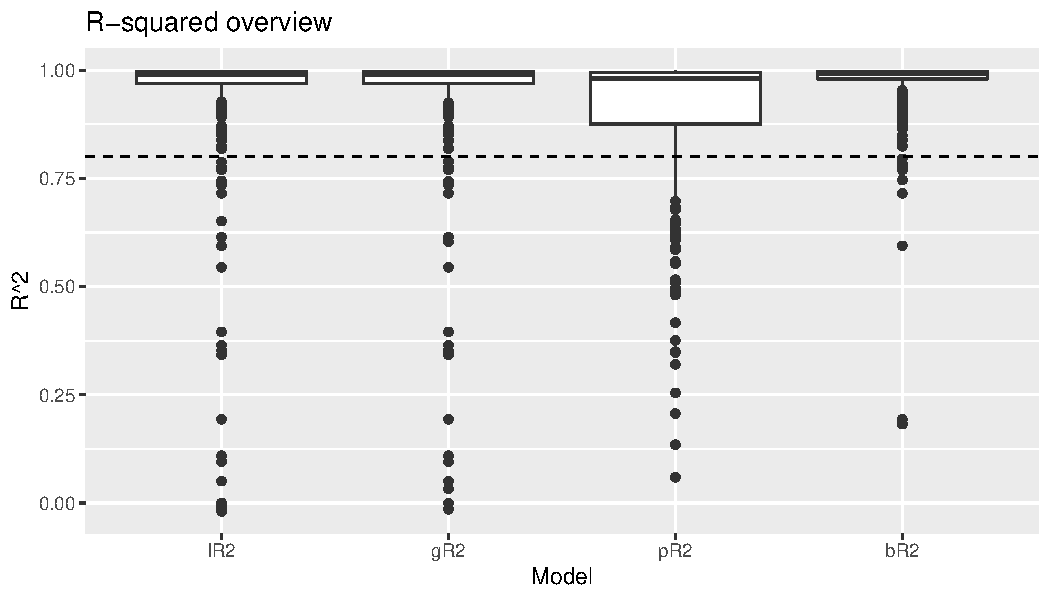
\includegraphics[width=0.9\textwidth]{../Results/anaPlots/r2snap.pdf}
    \caption{$R^2$ overview for each model, where $lR2=Logistic$, $gR2=Gompertz$, $pR2=Polynomial$, $bR2=Baranyi$}
    \label{fig:r2}
\end{figure}
\FloatBarrier
Figure \ref{fig:baddata} is an example of a data set where either all models' fit is bad($R^2 < 0.75$), or some of the model did not fit, and rest of the model indicated a bad fit. Before grading the model, data set groups that are similar to figure \ref{fig:baddata}, are excluded from the final evaluation data. Upon examination, all of these cases happened because the data set group itself is showing a bad shape, as could be seen in figure \ref{fig:baddata}. A total of 14 sets are excluded in this step, leaving the final count of data set groups to be 290. The majority of the data set groups are showing a good value in $R^2$, Which also indicates a pretty decent starting value choice.
\FloatBarrier
\begin{figure}[!htbp]
    \centering
    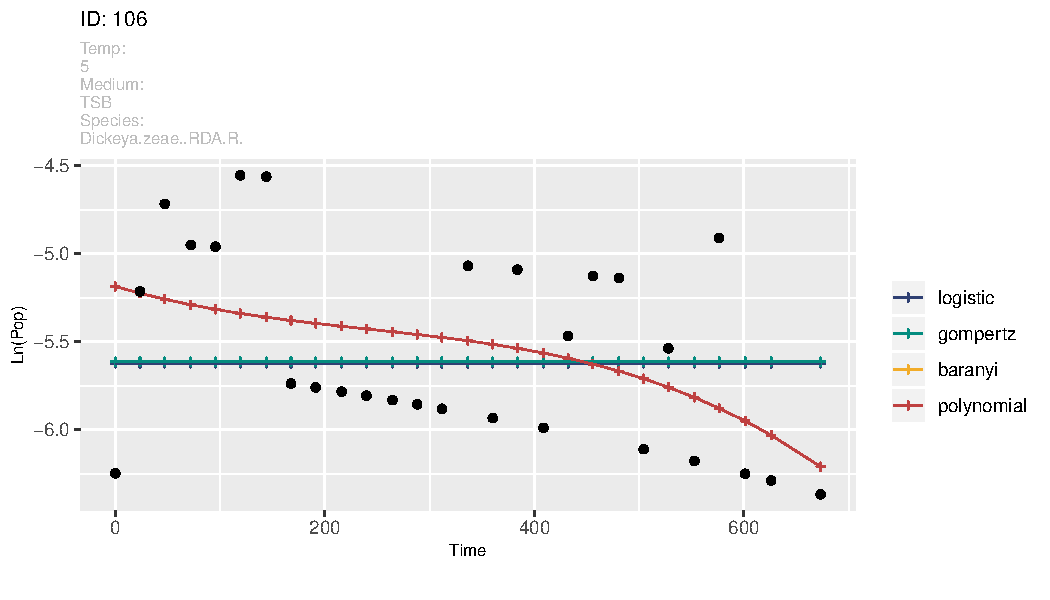
\includegraphics[width=0.9\textwidth]{../Results/allPlots/106.pdf}
    \caption{Example of deleted data set, where the Baranyi model didn't fit, and the rest three models showed bad fitting.}
    \label{fig:baddata}
\end{figure}
\FloatBarrier

\subsubsection{Grading}
This part will take the data set group $\mathit{ID}=92$ as an example to better illustrate the grading process. As can be seen in the evaluation matrix shown in table \ref{tab: evaluation} and graph shown in figure \ref{fig:gooddata} for this specific data group, all four model fit well(all with a $R^2>0.91$). And according to the rule for the grading system illustrated in section \ref{eq:aicweight}, only the Baranyi model gets 1 point for having a $\Delta AIC < 2$, and all other models would not get a point for all of their $\Delta AIC$ is greater than 2. As can be seen, $\Delta BIC$ in this particular study is giving the same results(all models have the same parameter count and fitting same data set group at a time), therefore $BIC$ would not be considered in the following analysis.

\FloatBarrier
\begin{table}[!htbp]
\begin{tabularx}{\linewidth}{X X X X X X X X}
\toprule & ${AIC}_\mathit{92}$ & ${\Delta}_\mathit{92} AIC$ & ${w}_\mathit{92} AIC$ &  ${BIC}_\mathit{92}$ & ${\Delta}_\mathit{92} BIC$ & $R^2$ & Point\\
\midrule
$Baranyi$ & -50.92886 & 0 & 9.996976e-01 & -48.98923 & 0 & 0.9942026 & 1 \\
$Gompertz$ & -33.33531 & 17.59355 & 1.511741e-04 & -31.39568 & 17.59355 & 0.9748831 & 0 \\
$Logistic$ & -33.33458 & 17.59428 & 1.511190e-04 & -31.39495 & 17.59428 & 0.9748816 & 0 \\
$Polynomial$ & -18.89898 & 32.02988 & 1.108328e-07 & -16.95935 & 32.02988 & 0.9163562 & 0\\
\bottomrule
\end{tabularx}
\caption{Evaluation matrix, ID=92}
\label{tab: evaluation}
\end{table}          
\FloatBarrier

\FloatBarrier
\begin{figure}[!htbp]
    \centering
    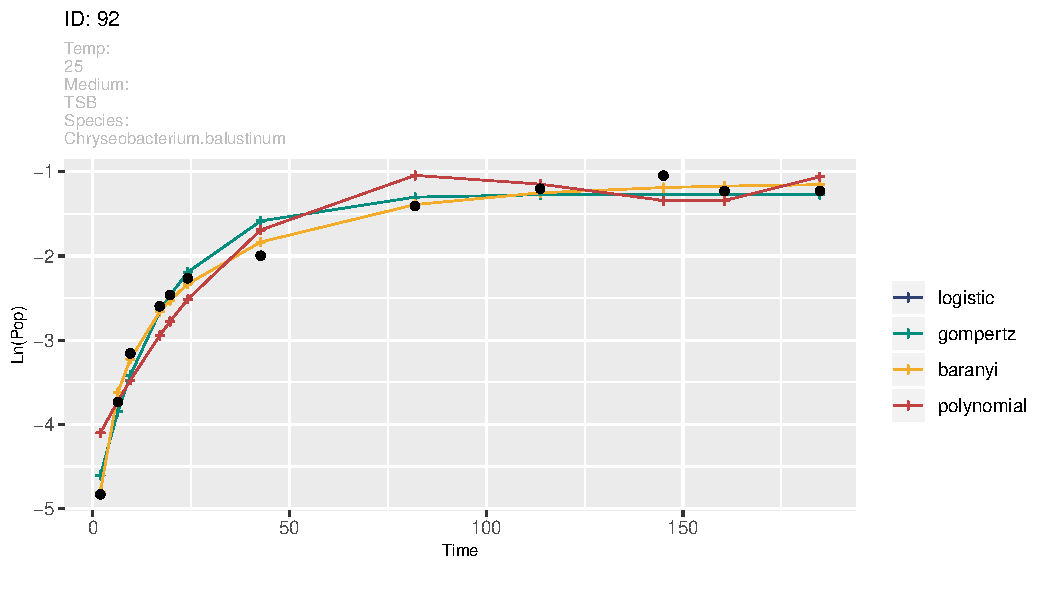
\includegraphics[width=0.9\textwidth]{../Results/allPlots/92.pdf}
    \caption{Example of a data set, where all models fit.}
    \label{fig:gooddata}
\end{figure}
\FloatBarrier

\subsection{Fit Result}
\subsubsection{Overall}
The final result for there models' fitting performances in the general data set can be seen in table \ref{tab: overallS}. The \textbf{Gompertz} model has the highest $P$ amongst all. It is the the best model for fitting this general data set, regarded as the best model to fit a data set group for a total of \textbf{182} times, taking up \textbf{62.5\%} of the total group size. The \textbf{Logistic} and \textbf{Baranyi} performed quite similarly with a percentage of \textbf{54.6} and \textbf{52.6} respectively.\\
\FloatBarrier
\begin{table}[!htbp]
\begin{tabularx}{\linewidth}{X X X X X}
\toprule Baranyi& \textbf{Gompertz} & Logistic & Polynomial & Total Groups\\
\midrule
 153(52.58\%) & \textbf{182(62.5\%)} & 159(54.6\%) & 77(24.6\%) & 291 \\
\bottomrule
\end{tabularx}
\caption{Overall Score, with percentage of Score over total size in bracket.}
\label{tab: overallS}
\end{table}          
\FloatBarrier

\subsubsection{ Co-variate Group Fit}
Upon further examination of the data set, \textbf{Tetraselmis tetrahele} is used to conduct the analysis of model's performance differences across temperature groups in the next section, as it is the only specie in the data set that allows such analysis(5 repetitions under same medium in different temperature groups). However, this part will only illustrate  the overall fit results in different temperature groups. The data set used for this study contains 17 temperature groups from 0 to 37$^\circ C$. The final fit result for each group using each model can be seen in table \ref{tab: tempfit}. \textbf{10 out of 17 (58.82\%)} groups, the \textbf{Gompertz} model still kept the lead amongst others. The \textbf{Logistic} and \textbf{Baranyi} performed quite similarly again, taking the lead for \textbf{5 out of 17(29.41\%)} and \textbf{6 out of 17(35.29\%)} groups respectively. 
\begin{table}[!htbp]
\begin{tabularx}{\linewidth}{X X X X X}
\toprule  Temperature($^\circ C$) & Baranyi & Gompertz & Logistic & Polynomial \\
\midrule
0 & 0 & \textbf{5} & 1 & 0  \\
2 & 5 & \textbf{8} & 7 & 5  \\
4 & \textbf{8} & 6 & 5 & 6  \\
5 & \textbf{13} & 11 & 12 & 7  \\
6 & 4 & 3 & \textbf{5} & 4  \\
7 & 4 & \textbf{14} & 6 & 2   \\
8 & 5 & \textbf{9} & 5 & 3  \\
10 & 10 & \textbf{18} & 11 & 4  \\
12 & \textbf{10} & 7 & 7 & 5  \\
15 & 24 & \textbf{29} & 24 & 14  \\
16 & 6 & 4 & \textbf{7} & 0  \\
20 & 19 & \textbf{21} & 20 & 15  \\
25 & \textbf{19} & 15 & 17 & 5  \\
30 & 7 & \textbf{9} & \textbf{9} & 4  \\
32 & \textbf{3} & \textbf{3} & \textbf{3} & 0  \\
35 & 14 & 16 & \textbf{17} & 3  \\
37 & 2 & \textbf{4} & 3 & 0  \\
\bottomrule
\end{tabularx}
\caption{Detailed point for temperature groups}
\label{tab: tempfit}
\end{table}          
\FloatBarrier

Fit results in data set groups with and without a death phase are illustrated in table \ref{tab: deathfit}. The \textbf{Gompertz} model performed the best in data set groups without a death phase with, and was out performed by \textbf{Baranyi} when there is a death phase.
\FloatBarrier
\begin{table}[!htbp]
\begin{tabularx}{\linewidth}{X X X X X}
\toprule  Death Phase & Baranyi & Gompertz & Logistic & Polynomial \\
\midrule
Yes & \textbf{19(73.1\%)} & 14(53.8\%) & 16(61.5\%) & 8(30.8\%)  \\
No & 134(52.3\%) & \textbf{168(63.4\%)} & 143(54.0\%) & 69(26.0\%)  \\
\bottomrule
\end{tabularx}
\caption{Detailed point for death phase groups, with percentage of the total group size following in brackets.}
\label{tab: deathfit}
\end{table}          
\FloatBarrier

\subsection{Comparisons In Performances}\label{comparison}
In order to have a more accurate and reasonable analysis on model's performance across different temperature groups, \textbf{Tetraselmis tetrahele} is chosen for this part of the analysis. A total of 5 temperature groups are presented($T=5$, $T=8$, $T=16$, $T=25$, $T=32$). Differences in the models performance which was indicated in $wAIC$ can be seen in figure \ref{fig:tempwaic}. Using the Kruskal-Wallis Test, All models have shown a significant differences (Baranyi $p-value = 0.001679$, Logistic $p-value = 0.01684$, Gompertz $p-value = 0.03801$, Polynomial $p-value = 0.01672$) in its $wAIC$ across different temperature groups at .05 significance level, indicating temperature may have affected these models' performance for this specific subset of data. The \textbf{Baranyi} have the most significant differences across all groups. \\ 
Further comparing the pairwise difference shows that the \textbf{Baranyi} has the most significant differences in pair 8$^\circ C$ - 16$^\circ C$($p-value = 0.007937$), the \textbf{Gompertz} has the most significant differences in pair 8$^\circ C$ - 25$^\circ C$($p-value = 0.01587$), the \textbf{Logistic} has the most significant differences in pair 8$^\circ C$ - 16$^\circ C$ and pair 5$^\circ C$ - 16$^\circ C$($p-value = 0.007937$), while the \textbf{Polynomial} has significant differences in pair 5$^\circ C$ - 16$^\circ C$, pair 8$^\circ C$ - 16$^\circ C$, and pair 16$^\circ C$ - 25$^\circ C$($p-value = 0.007937$).\\
\FloatBarrier 
\begin{figure}[!htbp]
    \centering
    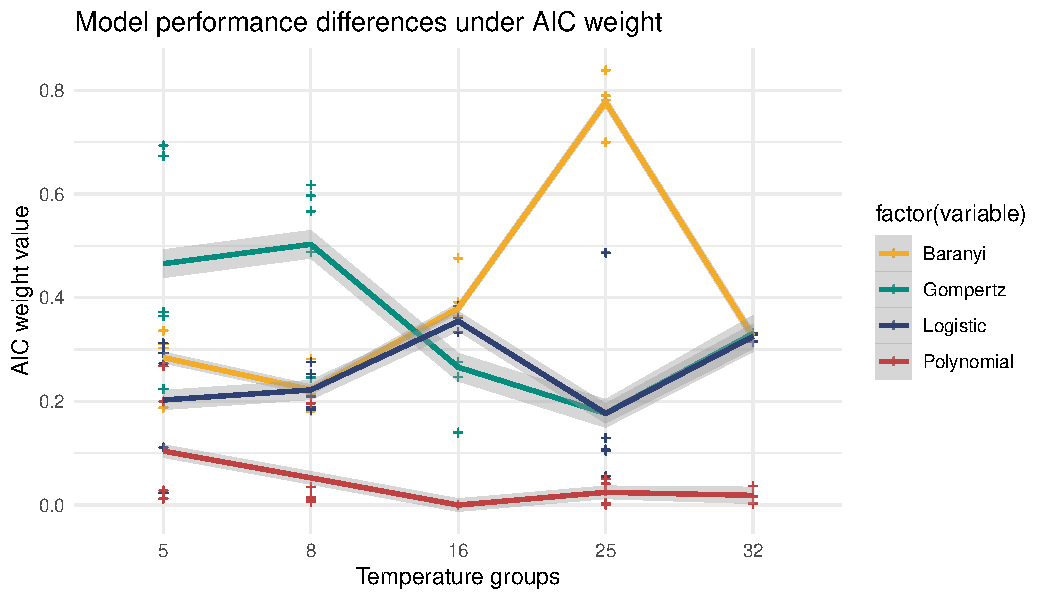
\includegraphics[width=0.9\textwidth]{../Results/anaPlots/wAICtemp.pdf}
    \caption{wAIC of different model across temperature groups, line with 2.5\% CI. }
    \label{fig:tempwaic}
\end{figure}
\FloatBarrier
Similarly for the death phase groups(seen in figure \ref{fig:deathphasewaic}), \textbf{Baranyi} and \textbf{Gompertz} model have shown a significant differences ($p-value = 0.04993$, $p-value = 0.02158$) in date set with and without a death phase at .05 significance level, suggesting that having a death phase in the data set group would probably affect these models' performances. The \textbf{Polynomial} and \textbf{Logistic} model have not shown a significant differences ($p-value = 0.6555$, $p-value = 0.8133$) in their performance across the two groups.
\FloatBarrier
\begin{figure}[!htbp]
    \centering
    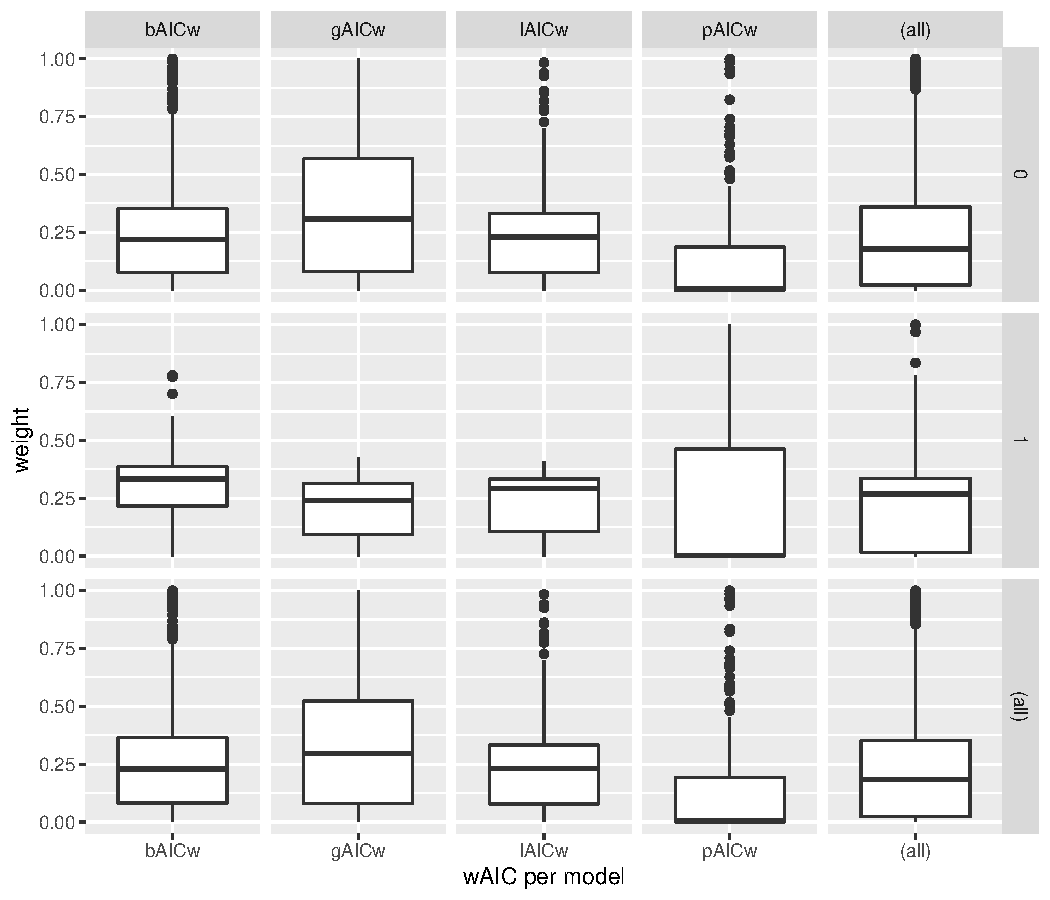
\includegraphics[width=0.7\textwidth]{../Results/anaPlots/wAICdeathphase.pdf}
    \caption{wAIC of different model for dataset with and without a death phase}
    \label{fig:deathphasewaic}
\end{figure}
\FloatBarrier

\section{Discussion}
\subsection{Reasons For Performance Difference}
Although the previous analysis has concluded there are performance differences for all four models, especially for the \textbf{Baranyi}, and some vague trends can be seen as in figure \ref{fig:tempwaic}, the results are only based on a rather small data subset($size = 92$) for \textbf{Tetraselmis tetrahele}. It is hardly an indication for anything solid.\\
Also, the difference could be caused by different sample sizes, measurement errors, and so on. However, these errors are very hard to quantify.\\
The fundamental question for model performance difference is probably much aligned with the fact on how temperature will affect the shape of the population growth curve for bacteria since models(excluding the \textbf{Polynomial}) used in this study indicate a very similar shape regardless.\\
A proper investigation in the relationship between temperature and models' performances or any other biological parameters like $r_{max}$ should require much more experimental data, and the analysis should be conducted on a larger scale to limit the error brought by the data.
\subsection{Death Phase And The Polynomial Model}
The \textbf{Polynomial}(Cubic) model is introduced to mainly illustrate the disadvantages other models have regarding the fourth stage of bacterial growth curves - death phase - since it allows the curve to have a decreasing phase after hitting the maximum point.\\
In reality, as shown in table \ref{tab: deathfit}, the behaviour of the Polynomial model is not better than any of the other models(Ranked the last). A closer look at a data set group that has a death phase(figure \ref{fig:deathphasedata}) may help to understand why it is the case.
\FloatBarrier
\begin{figure}[!htbp]
    \centering
    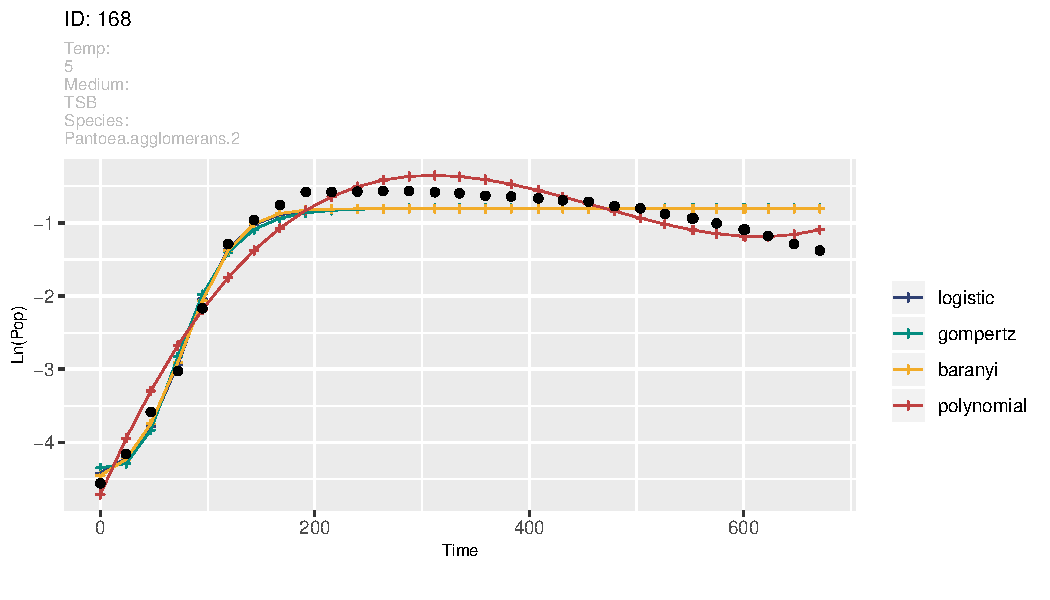
\includegraphics[width=0.9\textwidth]{../Results/allPlots/168.pdf}
    \caption{Example of a data set, where all models fit.}
    \label{fig:deathphasedata}
\end{figure}
\FloatBarrier
As can be seen, the data set group has shown a decline since $Time=200$, and models other than Polynomial are fitting the decline using a straight line. Although the Polynomial model is somehow catching the decline, the shape of the cubic model is relatively different from the 4-phased growth curve. Catching the decline in the data set group does not necessarily help with the overall fit result.\\
However, the comparison does show the disadvantages of the other three models used in this study at catching the decline after the peak. It also shows that the Polynomial model, due to its nature of having an increase after the decline, is not the best at fitting the death phase.\\
This could be a very rough first step of working on finding or building models that could work well for the 4-phased growth curve.
\subsection{Future Work}
There are more biology related analysis that could be done after understanding that the Gompertz model is the best model to use for this data set. An initial thought would be trying to understand the effect temperature has over $t_{lag}$ and $r_{max}$, since those are calculated each time the model fit a data set. A simple correlation and regression analysis could be done to understand the basic relationship, or using the new $time$ and $t_{lag}$, $time$ and $r_{max}$ data set, more models in relation to those variables could be bench-marked. However, since the focus of this study is fitting and comparing models for bacterial growth curves, those topics are not discussed.
\clearpage

\printbibliography
\end{document}